\section{Sheared Density Flow}
Consider the same velocity profile as  \eqref{ho:pro2} but with a
sheared density profile:
\begin{equation}\label{she1}
\rho =
\begin{cases}
\rho_0 &\text{if $z>0$,}\\
\rho_0+\Delta\rho &\text{if $z<0$,}\\
\end{cases}
\end{equation}
The trial solution is
\begin{equation}\label{she2}
\phi =
\begin{cases}
Ae^{-\alpha z} &\text{if $z>1$,}\\
Be^{-\alpha z} + Ce^{\alpha z} &\text{if $0<z<1$,}\\
De^{-\alpha z} + Ee^{\alpha z} &\text{if $-1<z<0$,}\\
Fe^{\alpha z} &\text{if $z<-1$.}
\end{cases}
\end{equation}
Using the same technique as last section, we get at $z=1$
\begin{equation}\label{she3}
    2(1-c)\alpha C=Be^{-2\alpha}+C
\end{equation}
and at $z=-1$
\begin{equation}\label{she4}
    2(1+c)\alpha D=D+Ee^{-2\alpha}
\end{equation}
However, the fluid near $z=0$ is affected by the buoyancy force due
to the density shearing, so I have to treat it with a different
method. First, by matching $\phi$, I get
\begin{equation}\label{she5}
    B+C=D+E
\end{equation}
Using the vorticity equation cited in Caulfield
\cite{Caulfield}\footnote{The result is following Hoiland, 1948.},
the $x$ component can be written as
\begin{equation}\label{she6}
    \frac{D}{Dt}\Bigl(\frac{\partial u}{\partial z}\Bigr)=
    \Bigl(g'\frac{\partial \xi}{\partial x}\Bigr)\delta(z-\xi)
\end{equation}
where $u=U(z)+u'$ is the total velocity in $x$ direction,
$g'=g\Delta\rho/\rho$ is the reduced gravitational acceleration,
$\xi$ is the perturbed displacement of the interface with density
jump $\Delta\rho$. Note that $U(0)=0$ at $z=0$ and linearizing, I
found that $u=u'$ and $D/Dt=\partial/\partial t$ at $z=0$. Integrate
\eqref{she6} over an arbitrary small region near the density
interface, I obtain
\begin{equation}\label{she7}
    \frac{\partial}{\partial t}(u'_+-u'_-)= g'\frac{\partial \xi}{\partial
    x}\quad \text{at $z=0$.}
\end{equation}
From \eqref{kh:b2},
\begin{equation}\label{she8}
\hat{\xi}=-\frac{\phi}{U-c}=\frac{\phi}{c}\quad\text{at $z=0$.}
\end{equation}
Recall that $u'=(d\phi/dz) e^{i\alpha( x - ct)}$ and $\xi=\hat\xi
e^{i\alpha( x - ct)}$, I can write \eqref{she7} in
\begin{align*}
    \frac{\partial}{\partial t}\Bigl[\frac{d(\phi_+-\phi_-)}{dz}e^{i\alpha( x - ct)}\Bigr]
    &= g'\frac{\partial}{\partial
    x}(\hat\xi e^{i\alpha( x - ct)})\\
    -i\alpha c[\alpha(-B+C+D-E)\phi e^{i\alpha( x - ct)}]
    &= g'(i\alpha\hat\xi e^{i\alpha( x - ct)})\\
    c\alpha(B-C-D+E)\phi &= g'\frac{\phi}{c}
\end{align*}
Define the bulk Richardson number as
\begin{equation}\label{she10}
    Ri_0=\frac{g\Delta\rho d}{\rho(\Delta u)^2}=\frac{g' 2}{2^2}=\frac{g'}{2}
\end{equation}
where $d$ is the thickness of the shear layer and $\Delta u$ is the
velocity difference of the upper and lower region. Finally I get
\begin{equation}\label{she11}
    B-C=D-E+\frac{2Ri_0}{\alpha c^2}
\end{equation}
Put together \eqref{she3}, \eqref{she4}, \eqref{she5} and
\eqref{she11}, we get the stability equation for a sheared density
flow:
\begin{equation}\label{she12}
\boxed{c^4+\Bigl(\frac{e^{-4\alpha}-(2\alpha-1)^2}{4\alpha^2}-\frac{Ri_0}{\alpha}\Bigr)c^2
+\frac{Ri_0}{\alpha}\Bigl(\frac{e^{-2\alpha}+(2\alpha-1)}{2\alpha}\Bigr)^2=0}
\end{equation}

The result is visualized by Lawrence et al.~\cite{Lawrence} in
Figure \ref{ho3}. The region I shows Kelvin-Helmholtz instability
while region II shows Holmboe instability.
\begin{figure}[htpb]
  \centering
  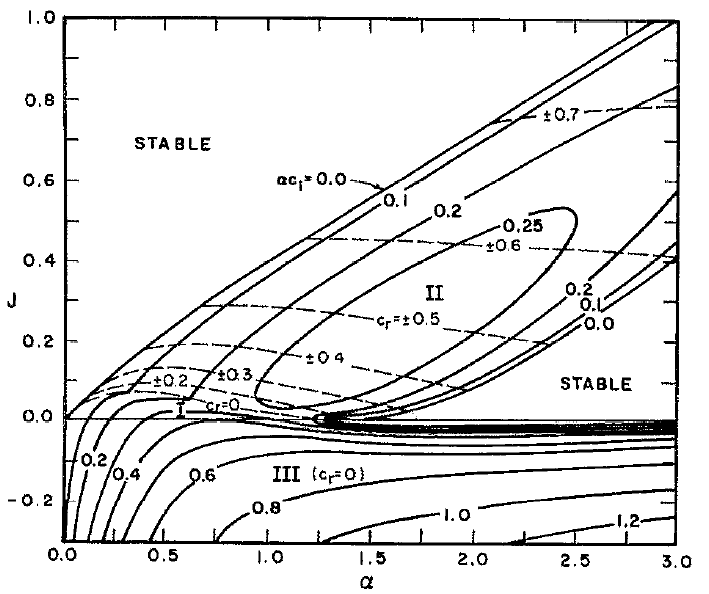
\includegraphics[width=0.9\textwidth]{ho3.png}\\
  \caption{Stability diagram for different $Ri_0$ and $\alpha$}\label{ho3}
\end{figure}
